\section{Zielsetzung}
\label{sec:Ziel}

In diesem Versuch sollen die Gesetze der Strahlenoptik für Reflexion, Brechung und Beugung von Licht verschiedener Wellenlängen überprüft werden.

\section{Theorie}
\label{sec:Theorie}
Das optische Spektrum reicht von ultraviolettem Licht mit einer Wellenlänge von $\SIrange{100}{380}{\nano\meter}$ bis hin zu infrarotem Licht mit einer Wellenlänge
von $\SI{780}{\nano\meter}$ bis $\SI{1}{\mm}$. Das menschliche Auge kann davon jedoch nur den Teilbereich von $\SIrange{380}{780}{\nano\meter}$ erfassen. \newline
Da Licht eine elektromagnetische Welle ist, lässt sich ihre Ausbreitung durch die Maxwell'schen Gleichung beschreiben. Für die Gesetze der Reflexion und der Brechung 
an Grenzflächen reichen aber auch die Gesetzmäßigkeiten der Strahlenoptik aus.\newline
Die Wellenausbreitung in der Strahlenoptik wird durch die Normale der Wellenfläche, die senkrecht auf der Wellenfront steht und Lichtstrahl genannt wird, ausgezeichnet.
Die Ausbreitungsgeschwindigikeit einer Lichtwelle ist in verschiedenen Medien unterschiedlich groß, weshalb sich das Licht bei einem Übergang von einem Material zu einem anderen zum Lot hin bricht.
Eine mathematische Beziehung liefert das Snellius'sche Brechungsgesetz
\begin{align}
    \label{eqn:snellius}
    n_1 \sin(\alpha)=n_2\sin(\beta).
\end{align}
Dabei sind $n_1$ und $n_2$ die Brechungsindizes des jeweiligen Materials, $\alpha$ der Einfalls- und $\beta$ der Ausfallswinkel.
Eine schematische Darstellung ist \autoref{fig:brechungBild} zu entnehmen. In der Abbildung trifft Licht aus einem optisch dünneren Medium, also einem Medium in dem sich eine Welle schneller bewegt,
auf ein optisch dichteres Medium, in dem Wellen langsamer sind.

\begin{figure}[H]
    \centering
    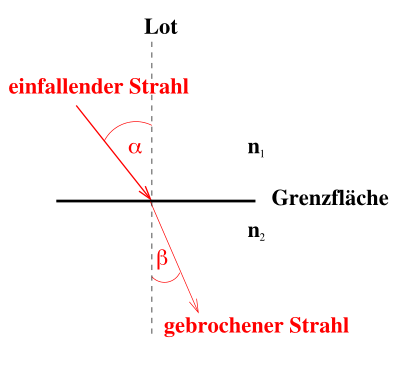
\includegraphics[width=0.5\textwidth]{data/brechung.png}
    \caption{Schematische Darstellung der Brechung eines Lichtstrahls zwischen zwei Medien\cite{Anleitung400}.}
    \label{fig:brechungBild}
\end{figure}

\noindent
Bei einem Prisma ist der Brechungswinkel von der Wellenlänge des Lichtes abhängig, was als Dispersion bezeichnet wird. Die Ablenkung $\delta$, die der Strahl beim Durchgang durch das Prisma erfährt,
wird durch die Gleichung
\begin{align}
    \delta = (\alpha_1+\alpha_2) - (\beta_1 + \beta_2)
    \label{eqn:prismaWinkel}
\end{align}
ausgedrückt. Eine schematische Darstellung des Strahlenganges von Licht durch ein Prisma ist in \autoref{fig:prismaBild} abgebildet.

\begin{figure}[H]
    \centering
    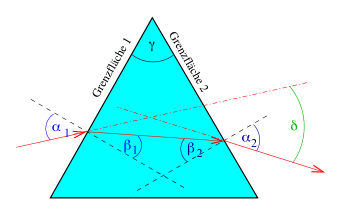
\includegraphics[width=0.5\textwidth]{data/prisma.png}
    \caption{Schematische Darstellung des Strahlenganges von Licht durch ein Prisma\cite{Anleitung400}.}
    \label{fig:prismaBild}
\end{figure}

\noindent
Neben der Brechung kann auch das Reflexionsgesetz mit der Strahlenoptik erklärt werden. Wenn ein Lichtstrahl auf eine Grenzfläche fällt, dann ist nach dem Reflexionsgesetz der Einfallswinkel $\alpha_1$ gleich dem Reflexionswinkel $\alpha_2$, also
\begin{align}
    \label{eqn:einfallAusfall}
    \alpha_1 = \alpha_2.
\end{align}
Eine schematische Darstellung des Phänomens ist \autoref{fig:reflexionBild} zu entnehmen. \newline

\begin{figure}[H]
    \centering
    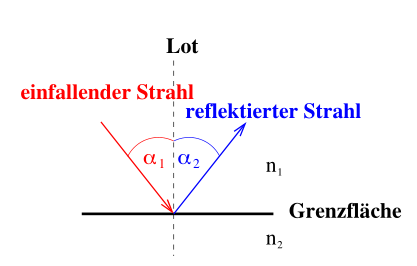
\includegraphics[width=0.5\textwidth]{data/reflexion.png}
    \caption{Schematische Darstellung der Reflexion eines Lichtstrahls zwischen zwei Medien\cite{Anleitung400}.}
    \label{fig:reflexionBild}
\end{figure}

\noindent
Da in der Regel, jedoch, ein Lichtstrahl an der Grenzfläche nicht vollständig reflektiert wird, gibt es noch einen Teil der in das Medium eindringt. Es gilt aber immer $R+T=1$.
In \autoref{fig:transmissionBild} ist das kombinierte Phänomen von Transmission und Reflexion dargestellt.

\begin{figure}[H]
    \centering
    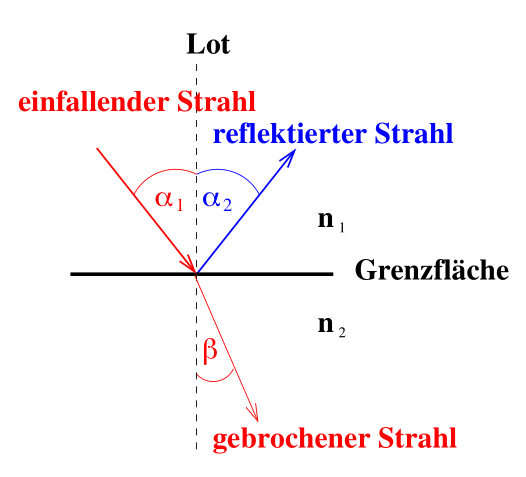
\includegraphics[width=0.5\textwidth]{data/transmission.png}
    \caption{Schematische Darstellung der Transmission und der Reflexion eines Lichtstrahls zwischen zwei Medien \cite{Anleitung400}.}
    \label{fig:transmissionBild}
\end{figure}

\noindent
Wenn Licht auf ein Hinderniss trifft, kann man allerding häufig beobachten, dass sich auch im geometrischen Schattenraum, also hinter dem Hinderniss, noch Licht befindet.
Dieses Phänomen wird als Beugung bezeichnet. Um dieses Auftreten zu erklären werden die Gesetze der Wellenoptik verwendet, da die Strahlenoptik keine ausreichende Erklärung liefert.  \newline
In der Wellenoptik findet vor allem das Huygens'sche Prinzip Anwendung, das besagt, dass jeder Punkt einer Welle der Ausgangspunkt einer Elementarwelle mit der gleichen Frequenz und Phase ist.
Die Einhüllende aller Elementarwellen ist wieder die urprünglich und stellt dessen Wellenfront auch zu einem späteren Zeitpunkt wieder dar.
Jedes Hinderniss im Strahlengang einer Welle, dessen Abmaße klein gegenüber der Wellenlänge ist, kann zur Beugung führen. \newline
Wenn sich überlagernde Wellen betrachtet werden, die dieselbe Frequenz und eine feste Phase besitzen, so ist zu beobachten, dass sie ein Interferenzbild erzeugen. Je nach
der gegenseitigen Phasenbeziehung können sie konstruktiv oder destruktiv miteinander Interferieren. Bei einem Gangunterschied von $\sfrac{\lambda}{2}$, also der halben Wellenlänge,
löschen sich die Wellen vollständig aus.
Wird eine Welle auf einen Spalt geworfen, so beugt sie sich in der Spaltöffnung. Gebeugte Wellen haben dieselbe Frequenz und eine feste Phase. Auf einem Schirm in einem Abstand $L$ vom Spalt mit der Spaltbreite $a$
ergibt sich ein Muster aus konstruktiver und destruktiver Interferenzstreifen. Die konstruktive Interferenz ist für Stellen mit dem Ausdruck
\begin{align}
    a\sin(\alpha)=k\lambda
    \label{eqn:spalt}
\end{align}
gegeben, wobei $\lambda$ die Wellenlänge des einfallenden Lichtes ist. Auf dem Schirm erscheint ein $k$-tes Maximum in einem Winkel $\alpha$ relativ zur geradlinigen Ausbreitunsrichtung.
Für ein Gitter aus $N$ Einfachspalten gleicher Breite mit der Gitterkonstanten $d$ folgt aus der Gleichung \eqref{eqn:spalt} eine Beziehung der Intensitätsmaxima bei einem Gitter zu
\begin{align}
    d\sin(\alpha)=k\lambda.
\end{align}